% This file was created with tikzplotlib v0.10.1.
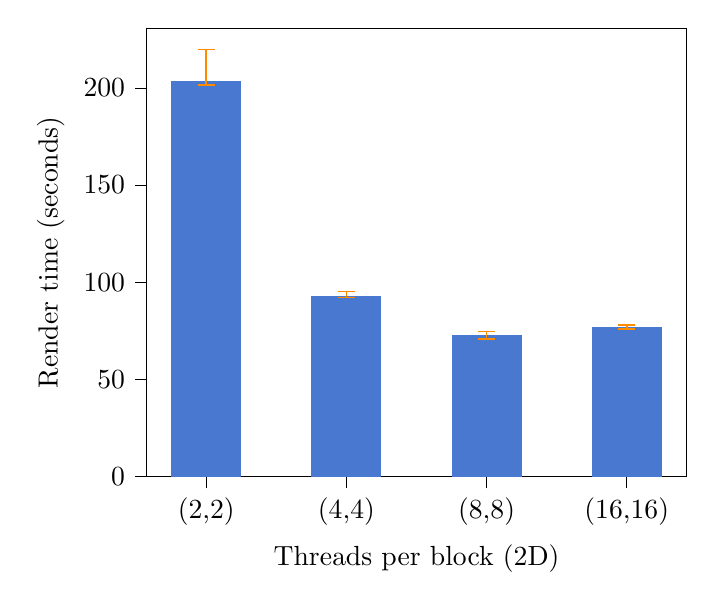
\begin{tikzpicture}

\definecolor{darkgray176}{RGB}{176,176,176}
\definecolor{darkorange}{RGB}{255,140,0}
\definecolor{royalblue72120207}{RGB}{72,120,207}

\begin{axis}[
tick align=outside,
tick pos=left,
x grid style={darkgray176},
xlabel={Threads per block (2D)},
xmin=-0.425, xmax=3.425,
xtick style={color=black},
xtick={0,1,2,3},
xtick={0,1,2,3},
xtick={0,1,2,3},
xticklabels={(2,2),(4,4),(8,8),(16,16)},
xticklabels={(2,2),(4,4),(8,8),(16,16)},
xticklabels={{(2,2)},{(4,4)},{(8,8)},{(16,16)}},
y grid style={darkgray176},
ylabel={Render time (seconds)},
ymin=0, ymax=230.72385,
ytick style={color=black}
]
\draw[draw=none,fill=royalblue72120207] (axis cs:-0.25,0) rectangle (axis cs:0.25,203.694);
\draw[draw=none,fill=royalblue72120207] (axis cs:0.75,0) rectangle (axis cs:1.25,92.906);
\draw[draw=none,fill=royalblue72120207] (axis cs:1.75,0) rectangle (axis cs:2.25,72.738);
\draw[draw=none,fill=royalblue72120207] (axis cs:2.75,0) rectangle (axis cs:3.25,77.155);
\path [draw=darkorange, semithick]
(axis cs:0,201.439)
--(axis cs:0,219.737);

\path [draw=darkorange, semithick]
(axis cs:1,92.183)
--(axis cs:1,95.289);

\path [draw=darkorange, semithick]
(axis cs:2,70.87)
--(axis cs:2,74.702);

\path [draw=darkorange, semithick]
(axis cs:3,75.957)
--(axis cs:3,77.988);

\addplot [semithick, darkorange, mark=-, mark size=3, mark options={solid}, only marks]
table {%
0 201.439
1 92.183
2 70.87
3 75.957
};
\addplot [semithick, darkorange, mark=-, mark size=3, mark options={solid}, only marks]
table {%
0 219.737
1 95.289
2 74.702
3 77.988
};
\end{axis}

\end{tikzpicture}
